%\setcounter{section}{-1}

\begin{wrapfigure}{r}{.52\textwidth}
\vspace{-1.15cm}
\begin{center}
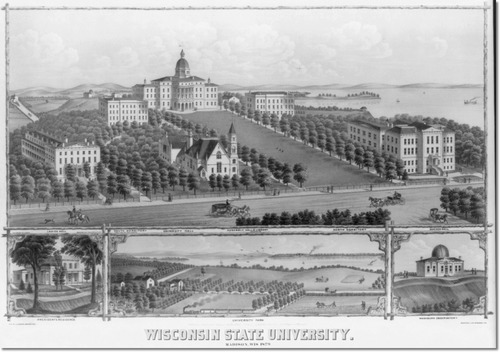
\includegraphics[width=.45\textwidth,trim=0 30 10 2, clip=true]{wisconsin-map}
\end{center}
\vspace{-.4cm}
\captionsetup{font=footnotesize,width=.52\textwidth}
\caption{A university campus.  Inset captions describe the buildings:
  ``\textsl{Ladies Hall}, \textsl{Dormitories}, \textsl{University
    Hall}, \textsl{Library} \textsl{and} \textsl{Assembly Hall},
  \textsl{Science Hall}, \textsl{President's Residence},
  \textsl{University Farm}, \textsl{Observatory}.''  This image serves
  as a key to the figures that illustrate our patterns.\label{madison-map}}
\vspace{-1.5cm}
\end{wrapfigure}

%OSS: Change abstract to free culture 
%OSS: New apporach? Put some things together that are not together elsewhere? Have an order and new look into this process
This paper  outlines an approach to the organization of learning that draws on the principles of free\slash libre\slash open source software (FLOSS), free culture, and peer production.
Mako Hill suggests that one recipe for success in peer production is to take a familiar idea -- for example, an encyclopedia -- and make it easy for people to participate in building it \cite[Chapter 1]{mako-thesis}.  We will take hold of ``learning in institutions'' as a map (Figure \ref{madison-map}), although it does not fully conform to our chosen tacitly-familiar territory of \emph{peeragogy}.  To be clear, peeragogy is for \emph{any group of people who want to learn anything}.\footnote{\url{https://www.youtube.com/watch?v=TDRGJzoNbAc}}

Although we are thinking about learning and adaptation that
may take place far outside of formal institutions, the historical
conception of a university helps give shape to our inquiry.
%
The model university is not separate from the life of the state or its
citizenry, but aims to ``assume leadership in the application of
knowledge for the direct improvement of the life of the people in
every sphere'' \cite[p.~88]{curti1949university}. Research that
\emph{adds to the store of knowledge} is another fundamental
obligation of the university \cite[p.~550]{curti1949university}.
While the university provides a familiar model for collaborative
knowledge work, it is not the only model available.
% wording issues here
Considering the role of collaboration in building reference resources,
Q\&A sites, and free\slash libre\slash open source software, we may
well ask: What would an accredited free\slash libre\slash open
university look like?  How would it compare or contrast with the
typical or stereotypical image in Figure
\ref{madison-map}?  Would it have similar structural features, like a
Library, Dormitory, Science Hall and so on?  Would participants take
on familiar roles \cite{corneli+crowdsourcing}?  How would it compare
with historical efforts like the Tuskegee Institute that involved
students directly in the production of physical infrastructure
\cite{washington1986up,building-peeragogy-accelerator}?

We use the word \emph{peeragogy} to talk about multi-way collaboration
in relatively non-hierarchical settings.  Examples are found in
education, but also in business, government, volunteer, and NGO
settings.  Peeragogy involves both problem solving and problem
definition, and results in learning.  Indeed, it is often preferable to
focus on solutions, since people know the ``problems'' all too well
\cite{ariyaratneXorganizationX1977}.  Participants in a peeragogical
endeavor collaboratively build emergent structures that are responsive
to their changing context, and that, in turn, change that context.  In
the Peeragogy project, we are developing the theory and practice of
peeragogy.

\emph{Design patterns} offer a methodological framework that we have
used to clarify our focus and organize our work.  A design pattern
expresses a commonly-occurring problem, a solution to that problem,
and rationale for choosing this solution \cite{meszaros1998pattern}.
This skeleton is typically fleshed out with a \emph{pattern template}
that includes additional supporting material; individual patterns are
connected with each other in a \emph{pattern language}.  What we
present here is rather different from previous pattern languages that touch
on similar topics -- like \emph{Liberating Voices}
\cite{schuler2008liberating}, \emph{Pedagogical Patterns}
\cite{bergin2012pedagogical}, and \emph{Learning Patterns}
\cite{iba2014learning}.  At the level of the pattern template, our
innovation is simply to add a ``What's next'' annotation, which
anticipates the way the pattern will continue to ``resolve''.

% The patterns we introduce here focus on negotiating the execution and implementation of solutions in their practical context.
%  This often requires compromise, adjustments and even restarts.  

This addition mirrors the central considerations of our approach, which is all about human interaction, and the challenges, fluidity and unpredictability that come with it.  Something that works for one person may not work for another or may not even work for the same person in a slightly different situation.  We need to be ready to clarify and adjust what we do as we go.   Even so, it is hard to argue with a sensible-sounding formula like ``If W applies, do X to get Y.'' In our view, other pattern languages often achieve this sort of common sense rationality, and then stop.  Failure in the prescriptive model only begins when people try to define things more carefully and make context-specific changes -- when they actually try to put ideas into practice.  The problem lies in the inevitable distance between \emph{do as I say}, \emph{do as I do}, and \emph{do with me} \cite[p.~26]{deleuze1994difference}.
%One is put in mind of Alfred Korzybski's famous remark: ``the map is not the territory.''   

%% Indeed, the strong version of our claim is that peeragogy is needed in applications of any map, blueprint, or design that seeks to involve people as people.
%% In some idealized sense, according to a certain school of thought, ``control'' is all that's required to move from a well-thought-out design to successful execution.  But, where do the designs come from in the first place \cite{von2003cybernetics}?
%% %
%% Moreover, once they exist, designs need to be interpreted, and often, revised.  
If people are involved, things get messy.   They may think that they are on the same page, only to find out that their understandings are wildly different.  For  example, everyone may agree that the group needs to go ``that way.''  But how far?  How fast?  It is rare for a project to be able to set or even define all of the parameters accurately and concisely at the beginning.
And yet design becomes a ``living language'' \cite[p.~xvii]{alexander1977pattern}  just insofar as it is linked to action.  Many things have changed since Alexander suggested that ``you will get the most `power' over the language, and make it your own most effectively, if you write the changes in, at the appropriate places in the book'' \cite[p.~xl]{alexander1977pattern}.  We see more clearly what it means to inscribe the changing form of design not just in the margins of a book, or even a shared wiki, but in the lifeworld itself.  Other recent authors on patterns share similar views \cite{reiners2012approach, schummer2014beyond,plast-project}.


%% We use the patterns of peeragogy to
%% \emph{constitute and occupy practical or speculative problems as such}
%% \cite[p.~204]{deleuze1994difference}.
%% %
%% Our patterns are a living language just insofar as they are linked to
%% action.

% Till Sch{\"u}mmer \emph{et al.}~have emphasized that pattern authors ``talk about what by definition is tacit'' and highlight the role of nonverbal communication ``needed to communicate the unspeakable'' \cite[p.~9]{schummer2014beyond}.

%% Whereas existing projects like Wikimedia's Wikiversity\footnote{\url{https://www.wikiversity.org/}} and the Peer-2-Peer University (P2PU) have created ``a model for lifelong learning alongside traditional formal higher education,''\footnote{\url{https://www.p2pu.org/en/}} they stop well short of offering accredited degrees.  

Learning and collaboration are of interest to both organizational studies and computer science, where researchers are increasingly making use of social approaches to software design and development, as well as agent-based models of computation \cite{minsky1967programming,poetry-workshop}.
%
The design pattern community in particular is very familiar with practices that we think of as peeragogical, including shepherding, writers workshops, and design patterns themselves \cite{harrison1999language,coplien1997pattern,meszaros1998pattern}.  We hope to help design pattern authors and researchers expand on these strengths.  The primary audience we envision for the paper are teams of people who aspire to collaboratively manage their own free/open/libre learning and development projects.

\subsection*{Plan of the work}

%This section will give the reader a sense of how the paper is organized. 

\begin{wraptable}{r}{.42\textwidth}
{\small
%
\vspace{-.3cm}
\begin{tabular}{|p{.4\textwidth}|}
\hline
\emph{Motivation} for using this pattern.\\ \hline
\end{tabular}
\vspace{-.12cm}

\begin{tabular}{|p{.4\textwidth}|}
\hline
\emph{Context} of application.\\ \hline
\emph{Forces} that operate within the context of application, each with a mnemonic glyph. \\ \hline
\emph{Problem} the pattern addresses.\\ \hline
\emph{Solution} to the problem.\\ \hline
\emph{Rationale} for this solution.\\ \hline
\emph{Resolution} of the forces, named in bold.\\ \hline
\end{tabular}
\vspace{.1cm}

%% \begin{tabular}{|p{.4\textwidth}|}
%% \hline
%% \emph{Inversion} Problems that could arise, and when \emph{not} to use the pattern.\\ \hline
%% \end{tabular}
%% \vspace{.1cm}

\begin{tabular}{|p{.4\textwidth}|}
\hline
\emph{Example 1}: How the pattern manifests in current Wikimedia projects.\\ \hline
\emph{Example 2}: How the pattern could inform the design of a future university.\\ \hline
\end{tabular}
\vspace{.1cm}

\begin{tabular}{|p{.4\textwidth}|}
\hline
\emph{What's Next in the Peeragogy Project}: How the pattern relates to our collective intention in the Peeragogy project\\ \hline
\end{tabular}
\vspace{-.1cm}
}
\captionsetup{font=footnotesize,width=.4\textwidth}
\caption{Pattern template.\label{tab:pattern-template}}
\vspace{-.9cm}
\end{wraptable}

Table \ref{tab:pattern-template} shows the pattern template that we use throughout the paper.  
Along with the traditional design patterns components \cite{meszaros1998pattern}, each of our patterns is fleshed out with two illustrative examples.  The first looks at how the pattern applies in current Wikimedia projects.  We selected Wikimedia as a source of examples because the project is familiar, a demonstrated success, and readily accessible.  The second example shows how the pattern could be applied in the design of a free\slash open\slash libre university.  Each pattern concludes with a boxed annotation that describes ``\emph{What's Next in the Peeragogy Project}''.
%
Following the convention of the design pattern literature, we write
the names of patterns in small-caps.  Section \ref{sec:Peeragogy}
defines the concept of \patternname{Peeragogy} more explicitly as a design pattern.  Sections
\ref{sec:Roadmap}--\ref{sec:Scrapbook} present the other patterns in
our pattern language.  This is followed by an emergent roadmap for the Peeragogy
project and a review of the broader contributions of this work.  Figure
\ref{fig:connections} illustrates the interconnections between the
patterns, and Table \ref{tab:core} summarizes their ``nuts and
bolts''.
% and which is followed by an emergent roadmap for the Peeragogy
%project and review of the contributions of this work as a whole.
%% , positioning this work as a
%% hands-on complement to existing sociological and historical research
%% about peer production (surveyed in \cite{benkler2015peer}).

%OSS: who cares? start w/example?
\subsection*{A short motivating example}
When one of us was a \patternname{Newcomer} to the Peeragogy project, she hit a wall in understanding the ``patterns'' section in the \emph{Peeragogy Handbook} v1.  A more seasoned peer invited her to a series of separate discussions with their own \patternname{Heartbeat} to flesh out the patterns and make them more accessible.  At that time the list of patterns was simply a list of paragraphs describing recurrent trends.  During those sessions, the impact and meaning of patterns captured her imagination.  She went on to become the champion for the pattern language and its application in the Peeragogy project.  During a ``hive editing'' session, she proposed the template we initially used to give structure to the patterns.  She helped further revise the pattern language for the \emph{Peeragogy Handbook}  v3, and attended PLoP 2015.  While a new domain can easily be overwhelming, this newcomer found \patternname{A specific project} to start with, and scaffolded her knowledge and contributions from that foundation.

\begin{table}[h]
{\small
\begin{tabular}{ll}
\begin{tabular}{@{\hspace{-.01\textwidth}}p{.25\textwidth}@{\hspace{-.00\textwidth}}p{.5\textwidth}}
\textbf{Pattern} & \textbf{How can we\ldots}\\
\patternname{Peeragogy} &~~\ldots find solutions together? \\
\patternname{Roadmap}&~~\ldots get everyone on the same page?\\
\patternname{Reduce, reuse, recycle}&~~\ldots avoid undue isolation?\\
\patternname{Carrying capacity}&~~\ldots avoid becoming overwhelmed?\\
\patternname{A specific project}&~~\ldots avoid becoming perplexed?\\
\patternname{Wrapper}&~~\ldots stay in touch?\\
\patternname{Heartbeat}&~~\ldots make the project ``real'' for participants?\\
\patternname{Newcomer}&~~\ldots make the project accessible to new people?\\
\patternname{Scrapbook}&~~\ldots maintain focus as time goes by?\\
\end{tabular}&
\begin{tabular}{@{\hspace{-.14\textwidth}}p{.5\textwidth}}
\textbf{Here's how:}\\
\emph{Figure out what the real problems are.}\\
\emph{Build a plan that we keep updating.}\\
\emph{Use what's there and share what we make.}\\
\emph{Clearly express when we're frustrated.}\\
\emph{Focus on concrete, doable tasks.}\\
\emph{Circulate any adjustments to the plan.}\\
\emph{Keep up a regular, sustaining rhythm.}\\
\emph{Let's learn together with newcomers.}\\
\emph{Keep coming back to the priorities.}\\
\end{tabular}\\
\end{tabular}
}
\caption{An overview of the problems and solutions in our pattern language.\label{tab:core}}
\end{table}
%\rule{0mm}{4.5cm}

\newpage

\afterpage{\clearpage}
\begin{figure}[p]
\vspace{-.9in}
{\centering
\begin{tikzpicture}[dot/.style={circle,inner sep=1pt,fill,name=#1}]
%\draw[step=1cm,gray,very thin] (0,0) grid (10,10);
\node (assess) at (5, 9.75) {{\Large {\sc Assess}}};
\node (organize) at (5, 0) {{\Large {\sc Organize}}};
\node (cooperate)[text width=2cm,align=center,rotate=270] at (10, 5) {{\Large {\sc Convene}}};
\node (convene)[text width=15cm,align=center,rotate=90] at (0, 5) {{\Large {\sc Cooperate}}};

\node(legend)[draw,rectangle,text width=2.67cm] at (9.25,.75) 
{\begin{tabular}{p{2.7cm}@{\hspace{-1mm}}}
\textbf{Legend}\\ \hline\vspace{-2mm} \textbf{A}\hspace{.41in}\textbf{B}\\
if pattern \textbf{A} refers to pattern \textbf{B}.
  \end{tabular}};
\draw[-{Latex[width=2mm]},draw=gray] ([xshift=5mm,yshift=1.75mm]legend.west) -- ([xshift=-14.8mm,yshift=1.75mm]legend.east);

%%%%%%%%%%%%%%%%%%%%%%%%%%%%%%%%%%%%%%%%%%%%%%%%%%%%%%%%%%%%%%%%%%%%%%%%%%%%%%%%%%%%%%%%%%%%%%%%%%%%%
\node[below = 5cm of assess] (roadmap) {\ref{sec:Roadmap}. \hyperref[sec:Roadmap]{\emph{Roadmap}}};
\node (reduce) at (5, 8.75) {\ref{sec:Reduce, reuse, recycle}. \hyperref[sec:Reduce, reuse, recycle]{\emph{Reduce, reuse, recycle}}};
\node (carryingcapacity) at (1.25, 7.15) {\ref{sec:Carrying capacity}. \hyperref[sec:Carrying capacity]{\emph{Carrying capacity}}};
\node[below = 3.2cm of carryingcapacity] (heartbeat) {\ref{sec:Heartbeat}. \hyperref[sec:Heartbeat]{\emph{Heartbeat}}};
\node (aspecificproject) at (8.5, 6.5) {\ref{sec:A specific project}. \hyperref[sec:A specific project]{\emph{A specific project}}};
\node[below = 1cm of roadmap] (wrapper) {\ref{sec:Wrapper}. \hyperref[sec:Wrapper]{\emph{Wrapper}}};
\node (newcomer) at (8.5, 3.25) {\ref{sec:Newcomer}. \hyperref[sec:Newcomer]{\emph{Newcomer}}};
\node[below = 1.7cm of wrapper] (scrapbook) {\ref{sec:Scrapbook}. \hyperref[sec:Scrapbook]{\emph{Scrapbook}}};
\node[above = 1cm of aspecificproject] (peeragogyproject) {\ref{sec:Peeragogy}. \hyperref[sec:Peeragogy]{\emph{Peeragogy}}};
%%%%%%%%%%%%%%%%%%%%%%%%%%%%%%%%%%%%%%%%%%%%%%%%%%%%%%%%%%%%%%%%%%%%%%%%%%%%%%%%%%%%%%%%%%%%%%%%%%%%%
\draw[-{Latex[width=2mm]},draw=gray] (peeragogyproject) -- (aspecificproject);
% \draw[-{Latex[width=2mm]},draw=gray] (aspecificproject) -- (par);
\draw[-{Latex[width=2mm]},draw=gray] (aspecificproject) -- (roadmap);
\draw[-{Latex[width=2mm]},draw=gray] (aspecificproject.230) to[out=250,in=40] (scrapbook);
\draw[-{Latex[width=2mm]},draw=gray] (aspecificproject) -- (carryingcapacity);
\draw[-{Latex[width=2mm]},draw=gray] (carryingcapacity.337) -- (newcomer);
\draw[-{Latex[width=2mm]},draw=gray] (carryingcapacity.330) -- (roadmap);
\draw[-{Latex[width=2mm]},draw=gray] (carryingcapacity) -- (peeragogyproject);
\draw[-{Latex[width=2mm]},draw=gray] ([xshift=1mm]carryingcapacity.south) -- (scrapbook.140);
% \draw[-{Latex[width=2mm]},draw=gray] ([xshift=2mm]creatingaguide.160) to[out=-215,in=-67] (carryingcapacity);
\draw[-{Latex[width=2mm]},draw=gray] (heartbeat) -- (aspecificproject.185);
\draw[-{Latex[width=2mm]},draw=gray] (heartbeat) -- (carryingcapacity);
\draw[-{Latex[width=2mm]},draw=gray] (heartbeat) -- (scrapbook.155);
\draw[-{Latex[width=2mm]},draw=gray] (heartbeat) -- (reduce.215);
\draw[-{Latex[width=2mm]},draw=gray] (newcomer) -- ([xshift=4mm]reduce.south);
\draw[-{Latex[width=2mm]},draw=gray] (newcomer) -- (aspecificproject);
% \draw[-{Latex[width=2mm]},draw=gray] (newcomer) -- (creatingaguide.north);
\draw[-{Latex[width=2mm]},draw=gray] (newcomer) -- (roadmap.350);
\draw[-{Latex[width=2mm]},draw=gray] (newcomer) -- (scrapbook.24);
% \draw[-{Latex[width=2mm]},draw=gray] (par) -- (scrapbook);
\draw[-{Latex[width=2mm]},draw=gray] (roadmap) -- (peeragogyproject.195);
\draw[-{Latex[width=2mm]},draw=gray] (roadmap.350) -- (newcomer);
\draw[-{Latex[width=2mm]},draw=gray] (roadmap) -- (wrapper);
\draw[-{Latex[width=2mm]},draw=gray] ([yshift=.3mm]roadmap.west) -- (heartbeat);
\draw[-{Latex[width=2mm]},draw=gray] (roadmap) -- (aspecificproject);
% \draw[-{Latex[width=2mm]},draw=gray] (scrapbook) -- (par);
\draw[-{Latex[width=2mm]},draw=gray] (scrapbook) -- (wrapper);
\draw[-{Latex[width=2mm]},draw=gray] (scrapbook.110) to[out=123,in=250] (reduce.245);
\draw[-{Latex[width=2mm]},draw=gray] (scrapbook.70) to[out=43,in=305] (roadmap.330);
% \draw[-{Latex[width=2mm]},draw=gray] ([xshift=2mm,yshift=-.4mm]reduce.south) -- (creatingaguide);
\draw[-{Latex[width=2mm]},draw=gray] (reduce) -- (carryingcapacity);
\draw[-{Latex[width=2mm]},draw=gray] (reduce) -- (roadmap);
\draw[-{Latex[width=2mm]},draw=gray] ([xshift=.7mm]wrapper.175) -- (heartbeat);
\draw[-{Latex[width=2mm]},draw=gray] ([xshift=-.7mm,yshift=-.3mm]wrapper.360) -- (newcomer);
\draw[-{Latex[width=2mm]},draw=gray] (wrapper) -- ([xshift=2.3mm]carryingcapacity.south);
\draw[-{Latex[width=2mm]},draw=gray] (wrapper) -- (roadmap);

\end{tikzpicture}


\par
}
\vspace{-.9in}
\caption{Connections between the patterns of peeragogy.  An arrow points from pattern \textbf{A} to pattern \textbf{B} if the text of the description of pattern \textbf{A} references pattern \textbf{B}.  Labels at the borders of the figure correspond to the main sections of the \emph{Peeragogy Handbook}.\label{fig:connections}}
\end{figure}
\FloatBarrier

\newpage

% deferring a more detailed elaboration of next steps in the educational arena to future work that will build on this basis.
% Technology has come a long way since Alexander suggested ``you will get the most `power' over the language, and make it your own most effectively, if you write the changes in, at the appropriate places in the book'' \cite[p.~xl]{alexander1977pattern}.
% While Christian Kohls insightfully describes patterns as the unique resolution of the dynamical forces acting in a given context \cite{kohls2010structure,kohls2011structure}.
%%% Patterns come to you through mindful awareness ... Charlotte: I think about patterns all the time now, I think about what makes me productive in a team.
% So, while we speak the same language as other developers of design patterns, our orientation is somewhat different, and our understanding of the word `pattern' is nuanced because we aim to take full account of the lifecycle of patterns.  Our work contributes to a recent ``performative'' turn \cite{schummer2014beyond}, which we believe gets at the heart of what design patterns can do.
%  
% In practical terms, we believe the patterns that we introduce here will be useful for students and educators who want their work to have real-world relevance, to activists and policy-makers who want to develop practicable solutions to large-scale problems, and to employees and managers who, like it or not, find themselves working in distributed teams. 

  
